% !TEX root = ../Dokumentation.tex
\subsection{Energieversorgung}
%
\textbf{Funktionsbeschrieb}\\[0.2cm]
Das autonome Entsorgungsfahrzeug muss mit Energie versorgt werden. Dazu werden Akkumulatoren eingesetzt, welche das Gerät während dem gesamten Einsatz mit Strom versorgen. 
\\[0.2cm]
\textbf{Komponentenbeschrieb}\\[0.2cm]
Um Störungen, die z.B. durch den erhöhten Anlaufstrom der Motoren verursacht werden könnten, zu vermeiden, werden die intelligenten Systeme (Microcontroller, Mini-Computer,etc.) möglichst getrennt von den Motoren gespiesen. Dazu werden zwei Lithium-Polymer-Akkumulatoren mit einer voraussichtlichen Spannung von 11.1 und 7.4 Volt verwendet, die galvanisch getrennt sind.
Der 11.1-Volt Akkumulator wird die Versorgung der Motoren gewährleisten und eine Kapazität von 2000-2400 mAh aufweisen. Für die empfindlicheren Systeme wird der 7.4 Volt LiPo zuständig sein, der eine Kapazität von 500-1000 mAh besitzt.
Die genaue Evaluation der Kapazitäten ist noch nicht abgeschlossen und bezieht sich lediglich auf die Resultate der Berechnungen, welche im Verlauf des Kapitels noch beschrieben werden.
\begin{figure}[H]
\centering
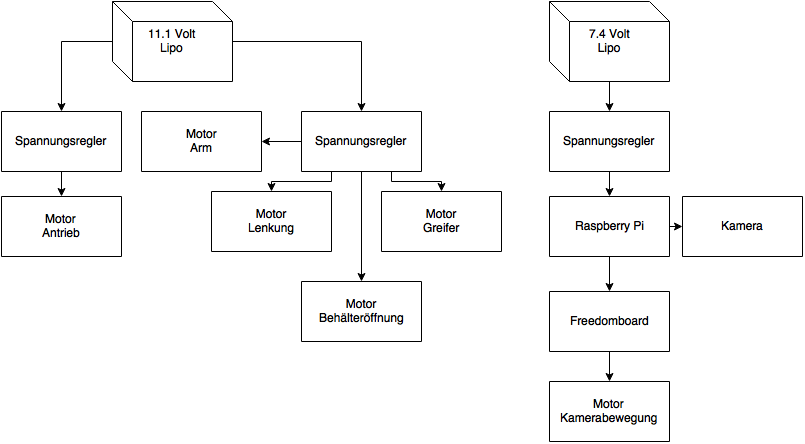
\includegraphics[width=0.8\textwidth]{03_Loesungskonzept/pictures/speisung.png}
\caption{Aufteilung der Akkumulatoren}	
\end{figure}
\textbf{Begründung}\\[0.2cm]
Die Entscheidung wird damit begründet, dass Lithium-Polymer-Akkumulatoren in einem vielfältigen Sortiment erhältlich sind und damit eine grosse Flexibilität bei der Auswahl ermöglichen. Somit würde sich auch die Suche nach einem Ersatz bei allfälligen Änderungen vereinfachen. Ausserdem weisen LiPos, im Vergleich zu anderen Akkumulatoren, eine wesentlich kompaktere Bauform auf, was entscheidend für die Auswahl war. \\[0.2cm]
\textbf{Berechnungen}\\[0.2cm]
Da die Wahl der Motoren noch nicht definitiv feststeht, wurden für die Berechnungen solche genommen, die den Anforderungen am nächsten kommen.\\
Leistungsberechnungen:
\begin{itemize}
\item Servomotor für die Lenkung:
\[
P=2\cdot \pi\cdot N\cdot M \to 2\cdot \pi\cdot 0.92\frac{U}{sec}\cdot 0.65Nm = 3.76W
\]
\item Servomotoren für Kamerabewegung und Greifer:
\[
P=2\cdot \pi\cdot N\cdot M \to 2\cdot \pi\cdot 0.72\frac{U}{sec}\cdot 0.18Nm = 0.81W
\]
\item Servomotor für den Greiferarm:
\[
P=2\cdot \pi\cdot N\cdot M \to 2\cdot \pi\cdot 1.14\frac{U}{sec}\cdot 0.32Nm = 2.5W
\]
\item DC-Motor für den Antrieb:
\[
P=2\cdot \pi\cdot N\cdot M \to 2\cdot \pi\cdot 5.258\frac{U}{sec}\cdot 2.23Nm = 73.98W
\]
\item DC-Motor für die Behälteröffnung:
\[
P=2\cdot \pi\cdot N\cdot M \to 2\cdot \pi\cdot 16.6\frac{U}{sec}\cdot 0.028Nm = 2.9W
\]
\end{itemize}
\newpage
Kapazitätenberechnungen:
\begin{itemize}
\item DC-Motor für den Antrieb:
\[
\frac{P\cdot t}{U} \to \frac{73.98W\cdot0.25h}{12V}= 1.54 Ah
\]
\item DC-Motor für die Behälteröffnung:
\[
\frac{P\cdot t}{U} \to \frac{2.9W\cdot0.25h}{4.8V}= 0.15 Ah
\]
\item Servomotor für die Lenkung:
\[
\frac{P\cdot t}{U} \to \frac{3.76W\cdot0.25h}{4.8V}= 0.19 Ah
\]
\item Servomotor für den Greiferarm:
\[
\frac{P\cdot t}{U} \to \frac{2.5W\cdot0.25h}{4.8V}= 0.13 Ah
\]
\item Servomotoren für Kamerabewegung und Greifer:
\[
\frac{P\cdot t}{U} \to \frac{0.81W\cdot0.25h}{4.8V}= 0.04 Ah
\]
\item Mini-Computer:
\[
I\cdot t \to 2A*0.25h = 0.5 Ah
\]
\item Benötigte Kapazität für den 11.1 Volt Akkumulator:
\[
1.54Ah+0.15Ah+0.19Ah+0.13Ah+0.04Ah = 2.05Ah
\]
\item Benötigte Kapazität für den 7.4 Volt Akkumulator:
\[
0.5Ah
\]
\end{itemize}
\subsubsection{Akkuüberwachung Schwellwertberechnung}
Damit die LiPo-Akkumulatoren nicht zerstört werden, muss sichergestellt werden das diese nicht tief entladen werden. Dies wird über das Freedomboard gelöst. Die Akkuspannung wird über einen Analog - Digitalwandler eingelesen. Wenn die Akkuspannung einen gewissen Wert unterschreiten, werden die Verbraucher an den Akkus "abgeschaltet". Eine Lipozelle sollte die Zellenspannung von 3.7V nicht unterschreiten. Im Normalfall sollten alle Zellen einzeln überwacht werden, dies ist jedoch im Rahmen dieses Prototypen nicht angemessen. Als Kompromiss wird gesamte Ausgangsspannung gemessen. Das heisst zwei beziehungsweise drei Zellen in Serie (je nach Akku).\\
Das Freedomboard kann nur Spannungen bis 3.3V einlesen. Daher ist ein Spannungsteiler nötig. Damit dieser Wert sicher nicht überschritten wird, wird mit einer maximal zulässigen Spannung von 3V gerechnet. Für UAkku wurde 13V gewählt, damit der AD-Wandler sicher nie 3V erreicht.\\
Für den 11.1V Akku:
\[	U_Akku/U_Frd=R1/R2\]
\[	13V/3V=4.33=g\]
Gewählt:
\[	R2=10k R1=R2*4.33=43kOhm\]
Der Abschaltwert des drei Zellen Akkus ist 3.7V * 3 = 11.1V.
Nach dem Spannungswandler entspricht dies einer Spannung von \[Uin/g=11.1V*10kOhm/(10kOhm+43kOhm)=2.075V\]
3.3V enspricht 65'535. Somit entspricht eine Spannung von 2.075V einem eingelesenen Spannungswert von 41592. Falls dieser Wert über längere (wenige Sekunden) unterschritten wird, wird eine Nachricht an das Raspberry gesendet und das System heruntergefahren.

Für den 7.1V (logik) Akku wurde mit einer maximale Spannung von 8.5V gerechnet:
\[	U_Akku/U_Frd=R1/R2\]
\[	8.5V/3V=2.83\]
Gewählt:
\[	R2=10k R1=R2*2.83=28.3kOhm\]
Für UAkku wurde 7.4V als Abschaltwert gewählt.\\
7.4V nach dem Spannungswandler entspricht einer Spannung von \[Uin/g=7.4V*10kOhm/(10kOhm + 28.3kOhm)=1.947\]
3.3V enspricht 65'535. Somit entspricht eine Spannung von 1.974V einem eingelesenen Spannungswert von 38673. Dieser Wert musste angepasst werden, da der Akku zu früh abschaltete, da unter Last die Akkuspannung kurzzeitig sinkt. Ausgehend von dem gemessenen Wert von 32158 und einer Akkuspannung von 7.55V wurde der neue Wert von 31513 berechnet.
\\[0.2cm]
\textbf{Vergleich Konzept und Umsetzung}\\[0.2cm]
Die Akkuüberwachung konnte einfacher realisiert werden, als es im Pren1 konzipiert war. Dies deshalb, weil bei der Energieversorung auf eine galvanische Trennung der beiden Akkumulatoren verzichtet wurde. Dies ermöglichte das direkte einlesen des Spannungswertes über einen Spannungsteiler. Geplant war ursprünglich eine Vergleicherschaltung mit einem Operationsverstärker für den 11.1V Akkumulator. Diese Vereinfachung war auch sicher ein Grund auf die galvanische Trennung zu verzichten.
